\section{General Information}

"Founded in 1901, NIST is a non-regulatory federal agency within the U.S. Department of Commerce. NIST's mission is to promote U.S. innovation and industrial competitiveness by advancing measurement science, standards, and technology in ways that enhance economic security and improve our quality of life" \cite{nist2016general}.
``NIST is one of the United States' oldest physical science laboratories. Congress established the agency to remove a major challenge to U.S. industrial competitiveness at the time — a second-rate measurement infrastructure that lagged behind the capabilities of the United Kingdom, Germany, and other economic rivals'' \cite{nist2016beta}.

``From the smart electric power grid and electronic health records to atomic clocks, advanced nanomaterials, and computer chips, innumerable products and services rely in some way on technology, measurement, and standards provided by the National Institute of Standards and Technology'' \cite{nist2016general}.

``Today, NIST measurements support the smallest of technologies to the largest and most complex of human-made creations — from nanoscale devices so tiny that tens of thousands can fit on the end of a single human hair up to earthquake-resistant skyscrapers and global communication networks'' \cite{nist2016beta}.

\clearpage

``NIST carries out its mission through the following programs:
\begin{itemize}
    \item the NIST laboratories, conducting world-class research, often in close collaboration with industry, that advances the nation's technology infrastructure and helps U.S. companies continually improve products and services;
    \item the Hollings Manufacturing Extension Partnership, a nation-wide network of local centers offering technical and business assistance to smaller manufacturers to help them create and retain jobs, increase profits, and save time and money; and
    \item the Baldrige Performance Excellence Program, which promotes performance excellence among U.S. manufacturers, service companies, educational institutions, health care provi\-ders, and nonprofit organizations; conducts outreach programs; and manages the annual Malcolm Baldrige National Quality Award which recognizes performance excellence and quality achievement.
\end{itemize}

NIST's financial year 2014 resources total \$850.0 million in direct appropriations, an estimated \$47.3 million in service fees, and \$107.0 million from other agencies'' \cite{nist2016general}.

``The agency operates in two main locations: Gaithersburg, Maryland (headquarters — 234-hectare campus — cf fig. \ref{fig:nist-gaithersburg-campus-map}) and Boulder, Colorado (84-hectare campus). NIST employs about 3,400 scientists, engineers, technicians, and support and administrative personnel. NIST also hosts about 2,700 associates from academia, industry, and other government agencies, who collaborate with NIST staff and access user facilities. In addition, NIST partners more than 1,300 manufacturing specialists and staff at more than 400 MEP service locations around the country'' \cite{nist2016general}.

``In addition, NIST jointly operates research organizations in four locations explicitly established to promote the kind of cross-disciplinary collaborations that accelerate research results'' \cite{nist2016locations}:

\begin{itemize}
    \item JILA, Boulder, Colo., a world-class physics research institute jointly operated by NIST and the University of Colorado at Boulder;
    \item Institute for Bioscience and Biotechnology Research (IBBR) (formerly CARB), Rockville, Md., an interdisciplinary partnership in cutting-edge biotechnology between NIST and the University of Maryland Biotechnology Institute;
    \item Joint Quantum Institute (JQI), College Park, Md., a new institute for advancing quantum physics research that is jointly operated with the University of Maryland;
    \item Hollings Marine Laboratory, Charleston, S.C., a national center for coastal ocean science, in which NIST is one of five federal, state, and university partners.
\end{itemize}

\begin{figure}[ht]
  \centering
  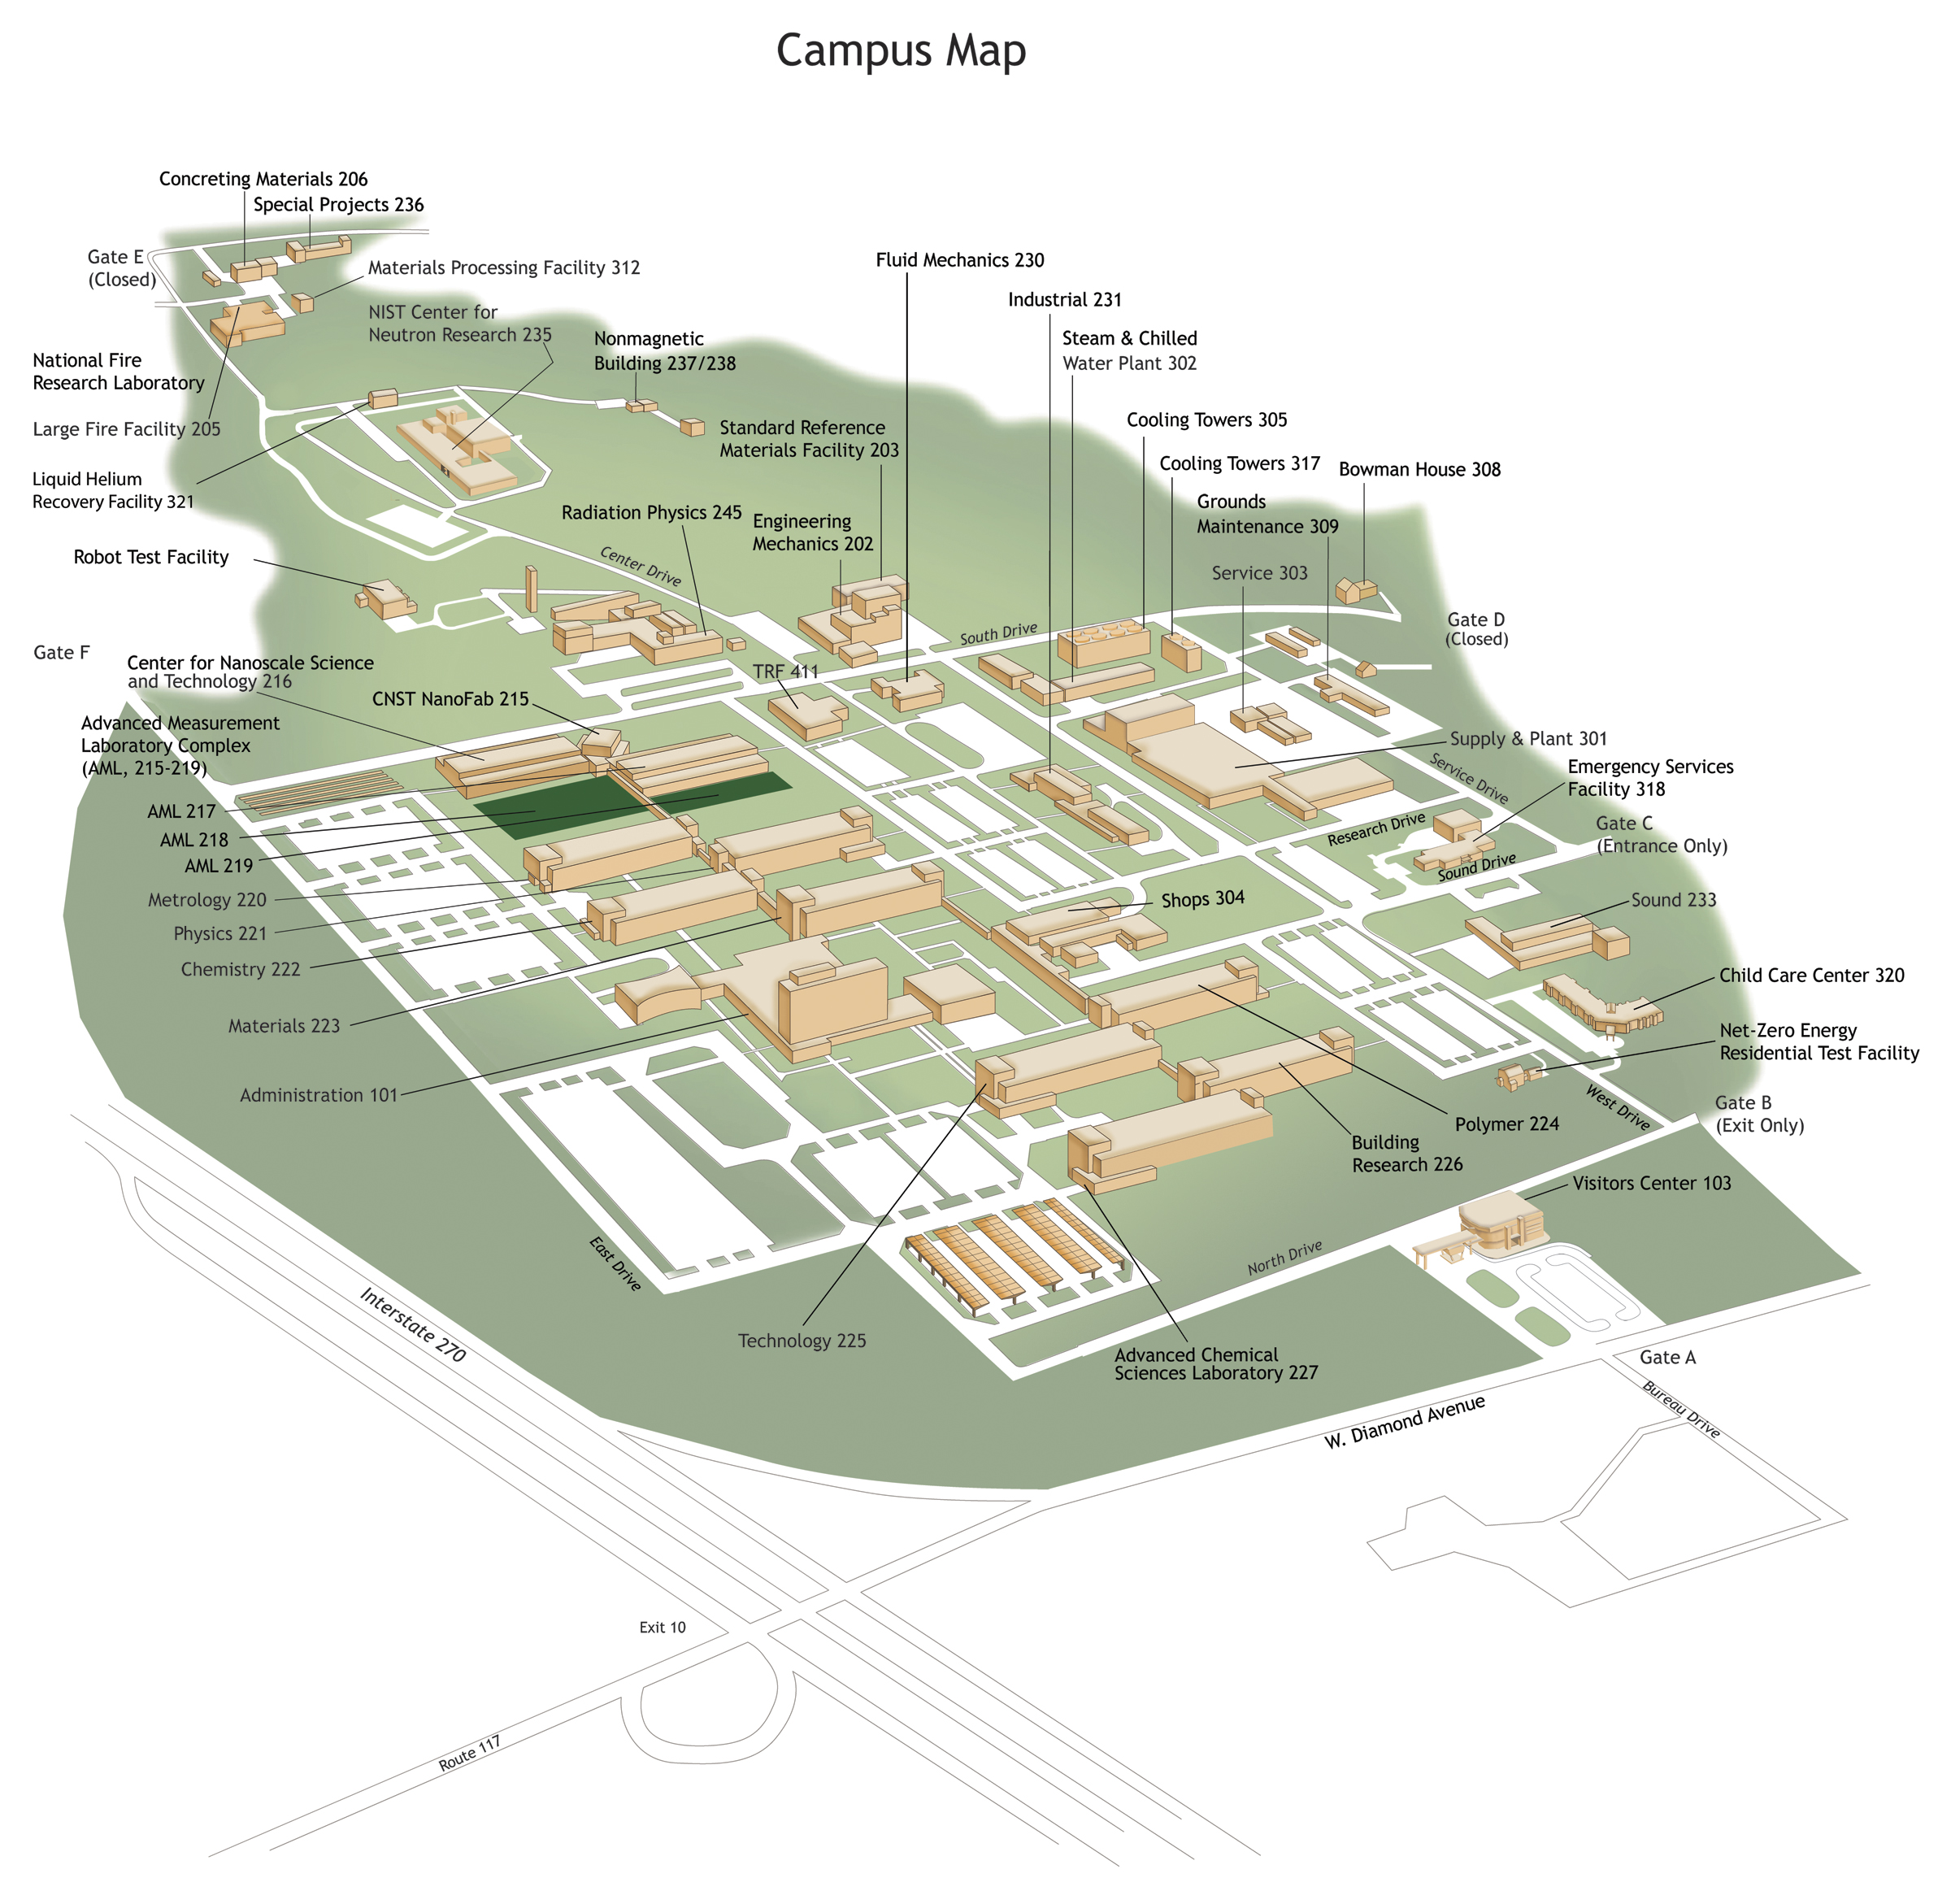
\includegraphics[scale=0.70]{figures/nist-gaithersburg-campus-map}
  \caption{NIST Gaithersburg Headquarters Campus Map}
  \label{fig:nist-gaithersburg-campus-map}
\end{figure}

\clearpage